\documentclass{beamer}

\usetheme{simple}

\usepackage{scalerel,xparse}
\usepackage{lmodern}
\usepackage[scale=2]{ccicons}
\usepackage{ulem}
\usepackage{tikz}
\usetikzlibrary{positioning,calc,automata}
\usepackage{algorithm}
\usepackage{algorithmic}
\usepackage{caption}

% Watermark background (simple theme)
\setlength{\parindent}{0cm}
\setwatermark{\includegraphics[height=8cm]{img/chungus.png}}


\title{\sout{CSC363H5} CSC258H5 Tutorial 1}
\subtitle{Paul's Revenge}
\date{\today}
\author{Paul ``sushi{\textunderscore}enjoyer'' Zhang}
\institute{University of Chungi}


\NewDocumentCommand\emojisushi{}{
    \includegraphics{img/1f363.png}
}
\NewDocumentCommand\emojifish{}{
    \includegraphics{img/1f41f.png}
}
\NewDocumentCommand\emojirice{}{
    \includegraphics{img/1f35a.png}
}
\NewDocumentCommand\emojisavouring{}{
    \includegraphics[scale=0.2]{img/1f60b.png}
}

\begin{document}

\maketitle

\begin{frame}{Learning objectives this tutorial}
By the end of this tutorial, you should...
\begin{itemize}
\item Be able to name the TA and his favourite food. This is where your tuition is going.
\item Have become good friends with everyone in this tutorial session.
\item Be able to describe what a URM is, and relate it to your knowledge of assembly programming (if you've done that before).
\item Be able to create URMs that perform operations such as addition.
\item Grasp the idea of a Turing Machine at a very informal level.
\item Appreciate the computational power of the personal computer, but realize that it only can do the things that a Turing machine can, which can only do things that a URM can.
\item See \texttt{helo{\textunderscore}fish.jpg} in your dreams.
\item Have a proof for P = NP, the Riemann hypothesis, and have attained nirvana. 
\end{itemize}
\end{frame}

\begin{frame}{helo!}
Welcome to CSC363! Here's \texttt{helo{\textunderscore}fish.jpg}.
\begin{figure}
\includegraphics[scale=0.2]{img/helo_fish.jpg}
\end{figure}
\texttt{helo{\textunderscore}fish.jpg} shall revisit my tutorial from time to time. Today, \texttt{helo{\textunderscore}fish.jpg} sends her greetings and hopes she will not haunt your dreams. 

  \begin{columns}
    \column{.5\textwidth}
    \texttt{helo{\textunderscore}fish.jpg} will say goodbye for now. Say your farewells!

    \column{.5\textwidth}
      \begin{block}{Protip...}
         \texttt{helo{\textunderscore}fish.jpg} wants you to make friends in this tutorial session! Say hi to the people sitting right beside you.
      \end{block}
  \end{columns}
  
\end{frame}

\begin{frame}{a bit about myself, i guess?}
Hai! I'm paul (he/him), B.Sc., M.Sc, Ph.D, D.P.H, S.Sc.D, and others (in minecraft). Address me however you'd like!

\vspace{2mm}

I'm doing a mathematics specialist (i'm done my cs minor).

My favourite ice cream flavour is coffee.

\vspace{2mm}

Current status: sad and alone in downtown toronto with nae pals ;-;
kinda lonely from time to time, wanna chat with me? owo
\begin{itemize}
\item office hours: Wed 5-6pm (after this tut), same zoom link
\item email: \texttt{pol.zhang@mail.utoronto.ca}
\item discord: \texttt{sjorv\#0943}
\item website: \url{https://sjorv.github.io/} (not finished yet sowwy)
\item reddit: guess lol
\item facebook/instagram/twitter/whatsapp/tiktok/snapchat/\\
vkonkakte/line/amazon/quercus/tinder/chungustalk: nope, sorry :((
\end{itemize}
  
\end{frame}

\begin{frame}{Oh yea, i just realized something...}
When making those slides, I realized that for people enrolled in the Friday lecture, you will be attending this tutorial before you have learned any course content.

\vspace{2mm}

I've tried to make the slides as self-contained as possible, so you don't need knowledge from the lecture. But if I have any gaps (or you have questions), please don't hesi\textbf{taste} to ask! owo

\vspace{2mm}

Also, we are doing some really \textbf{low level} ``programming'' stuff today. Knowledge of assembly language is not required by any means, but if you've done assembly programming before it might help to relate today's content to it.
\end{frame}

\begin{frame}{What's a URM?}
If you recall from class, we wanted to mathematically define what it means for a function to be ``computable''. For simplicity, we only consider functions $f: \mathbb N^k \to \mathbb N$ for now.

\vspace{4mm}

A \textbf{U}niform \textbf{R}esource \textbf{M}achine is one way to formally define computability of functions.


\end{frame}

\begin{frame}{What's a URM?}
Consider a ``tape'' that extends infinitely in one direction. This tape can be thought of as memory in a computer (except we have infinite memory).

\vspace{2mm}

We will label the positions on the tape (or \textit{registers}) $R_1, R_2, \ldots$. Each register can store a \textbf{natural} number (including 0).
\begin{center}
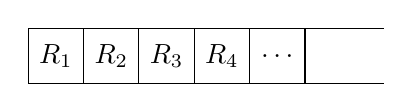
\begin{tikzpicture}[every node/.style={block},
        block/.style={minimum height=2em,minimum width=2em,outer sep=0pt,draw,rectangle,node distance=0pt}]
   \node (R1) {$R_1$};
   \node (R2) [right=of R1] {$R_2$};
   \node (R3) [right=of R2] {$R_3$};
   \node (R4) [right=of R3] {$R_4$};
   \node (R5) [right=of R4] {$\ldots$};
   \draw (R5.north east) -- ++(1cm,0) (R5.south east) -- ++ (1cm,0);
\end{tikzpicture}
\end{center}

We will manipulate the values on the tape according a series of instructions, called a \textit{URM program}. The instructions are very similar to assembly programming if you have done it before.
\end{frame}

\begin{frame}{What's a URM?}
A URM program consists of a series of \textit{basic instructions}. The instructions are numbered $1, 2, \ldots, m$, where $m$ is the number of instructions the URM program has.

\vspace{2mm}

There are four basic instructions:
\begin{itemize}
\item The zero instruction $Z(n)$: replace the number in $R_n$ (the $n$th position on the tape) with 0.
\item The successor instruction $S(n)$: Add 1 to the number in $R_n$ (i.e. increment it).
\item The copy instruction $C(m, n)$: Replace the number in $R_n$ with the number in $R_m$. This does not affect $R_m$.
\item The jump instruction $J(m, n, q)$: If the numbers in $R_m$ and $R_n$ are equal, go to instruction $q$ (otherwise go to the next instruction).\footnote{If $q > m$ (so the $q$th instruction doesn't exist), halt.}
\end{itemize}
\end{frame}

\begin{frame}{What's a URM?}
The URM takes in a $k$-tuple $(a_1, a_2, \ldots, a_k) \in \mathbb N^k$ as input.

\vspace{2mm}

We start with values $a_1$ in $R_1$, $a_2$ in $R_2$, and so on, until $a_k$ in $R_k$. For $i > k$, $R_i$ starts with $0$ (so all the other registers start as 0).

\begin{center}
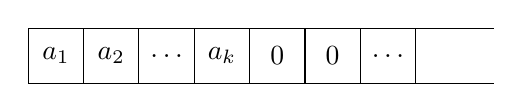
\begin{tikzpicture}[every node/.style={block},
        block/.style={minimum height=2em,minimum width=2em,outer sep=0pt,draw,rectangle,node distance=0pt}]
   \node (R1) {$a_1$};
   \node (R2) [right=of R1] {$a_2$};
   \node (R3) [right=of R2] {$\ldots$};
   \node (R4) [right=of R3] {$a_k$};
   \node (R5) [right=of R4] {$0$};
   \node (R6) [right=of R5] {$0$};
   \node (R7) [right=of R6] {$\ldots$};
   \draw (R7.north east) -- ++(1cm,0) (R7.south east) -- ++ (1cm,0);
\end{tikzpicture}
\end{center}

\vspace{2mm}

Then the URM executes its instructions in order.

\vspace{2mm}

The output of the URM is a natural number: whatever number remains in $R_1$ at the end of execution is the output. 

\vspace{2mm}

\underline{Note that some URMs don't terminate (in the case of a loop).}
\end{frame}

\begin{frame}{What's a URM?}
Then, we can say a function $f: \mathbb N^k \to \mathbb N$ is \textit{computable} if there exists a URM $M$ such that for any input $(a_1, \ldots, a_k) \in N^k$, $M$ terminates on input $(a_1, \ldots, a_k)$ and outputs $f(a_1, \ldots, a_k)$.
\end{frame}

\begin{frame}{Example}
Let $f$ be the function that adds two natural numbers:
$$f: \mathbb N^2 \to \mathbb N, f(a, b) = a + b.$$

We construct a URM that computes $f$.

\vspace{4mm}

URM instructions:
\begin{algorithmic}[1]
\STATE {$J(2, 3, 69420)$}
\STATE {$S(1)$}
\STATE {$S(3)$}
\STATE {$J(1, 1, 1)$}
\end{algorithmic}
Note if the numbers in $R_2$ and $R_3$ are equal, $J(2, 3, 69420)$ points to a nonexistent instruction and therefore halts execution. $J(1, 1, 1)$ jumps to instruction $1$ unconditionally.
\end{frame}

\begin{frame}{Example}
\begin{algorithmic}[1]
\STATE {$J(2, 3, 69420)$}
\STATE {$S(1)$}
\STATE {$S(3)$}
\STATE {$J(1, 1, 1)$}
\end{algorithmic}
On input $(3, 2)$, we start with the following tape:
\begin{center}
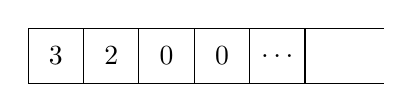
\begin{tikzpicture}[every node/.style={block},
        block/.style={minimum height=2em,minimum width=2em,outer sep=0pt,draw,rectangle,node distance=0pt}]
   \node (R1) {$3$};
   \node (R2) [right=of R1] {$2$};
   \node (R3) [right=of R2] {$0$};
   \node (R4) [right=of R3] {$0$};
   \node (R5) [right=of R4] {$\ldots$};
   \draw (R5.north east) -- ++(1cm,0) (R5.south east) -- ++ (1cm,0);
\end{tikzpicture}
\end{center}
We start executing from line 1: $J(2, 3, 69420)$. Nothing happens since $2 \neq 0$.
\begin{center}
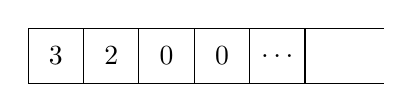
\begin{tikzpicture}[every node/.style={block},
        block/.style={minimum height=2em,minimum width=2em,outer sep=0pt,draw,rectangle,node distance=0pt}]
   \node (R1) {$3$};
   \node (R2) [right=of R1] {$2$};
   \node (R3) [right=of R2] {$0$};
   \node (R4) [right=of R3] {$0$};
   \node (R5) [right=of R4] {$\ldots$};
   \draw (R5.north east) -- ++(1cm,0) (R5.south east) -- ++ (1cm,0);
\end{tikzpicture}
\end{center}

\end{frame}

\begin{frame}{Example}
\begin{columns}
\column{0.5\linewidth}
\begin{center}
\begin{algorithmic}[1]
\STATE {$J(2, 3, 69420)$}
\STATE {$S(1)$}
\STATE {$S(3)$}
\STATE {$J(1, 1, 1)$}
\end{algorithmic}
\end{center}
\column{0.5\linewidth}
\begin{center}
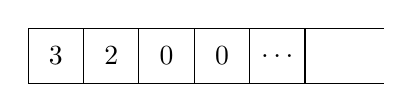
\begin{tikzpicture}[every node/.style={block},
        block/.style={minimum height=2em,minimum width=2em,outer sep=0pt,draw,rectangle,node distance=0pt}]
   \node (R1) {$3$};
   \node (R2) [right=of R1] {$2$};
   \node (R3) [right=of R2] {$0$};
   \node (R4) [right=of R3] {$0$};
   \node (R5) [right=of R4] {$\ldots$};
   \draw (R5.north east) -- ++(1cm,0) (R5.south east) -- ++ (1cm,0);
\end{tikzpicture}
\end{center}
2: $S(1)$
\begin{center}
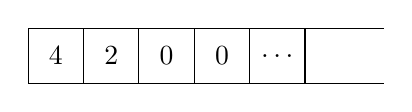
\begin{tikzpicture}[every node/.style={block},
        block/.style={minimum height=2em,minimum width=2em,outer sep=0pt,draw,rectangle,node distance=0pt}]
   \node (R1) {$4$};
   \node (R2) [right=of R1] {$2$};
   \node (R3) [right=of R2] {$0$};
   \node (R4) [right=of R3] {$0$};
   \node (R5) [right=of R4] {$\ldots$};
   \draw (R5.north east) -- ++(1cm,0) (R5.south east) -- ++ (1cm,0);
\end{tikzpicture}
\end{center}
3: $S(3)$
\begin{center}
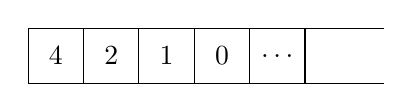
\begin{tikzpicture}[every node/.style={block},
        block/.style={minimum height=2em,minimum width=2em,outer sep=0pt,draw,rectangle,node distance=0pt}]
   \node (R1) {$4$};
   \node (R2) [right=of R1] {$2$};
   \node (R3) [right=of R2] {$1$};
   \node (R4) [right=of R3] {$0$};
   \node (R5) [right=of R4] {$\ldots$};
   \draw (R5.north east) -- ++(1cm,0) (R5.south east) -- ++ (1cm,0);
\end{tikzpicture}
\end{center}
\end{columns}
\end{frame}

\begin{frame}{Example}
\begin{columns}
\column{0.5\linewidth}
\begin{center}
\begin{algorithmic}[1]
\STATE {$J(2, 3, 69420)$}
\STATE {$S(1)$}
\STATE {$S(3)$}
\STATE {$J(1, 1, 1)$}
\end{algorithmic}
\end{center}
\column{0.5\linewidth}
\begin{center}
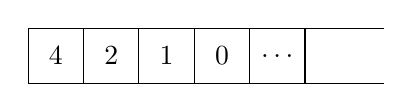
\begin{tikzpicture}[every node/.style={block},
        block/.style={minimum height=2em,minimum width=2em,outer sep=0pt,draw,rectangle,node distance=0pt}]
   \node (R1) {$4$};
   \node (R2) [right=of R1] {$2$};
   \node (R3) [right=of R2] {$1$};
   \node (R4) [right=of R3] {$0$};
   \node (R5) [right=of R4] {$\ldots$};
   \draw (R5.north east) -- ++(1cm,0) (R5.south east) -- ++ (1cm,0);
\end{tikzpicture}
\end{center}
4: $J(1, 1, 1)$

1: $J(2, 3, 69420)$

2: $S(1)$
\begin{center}
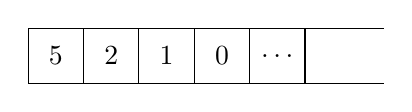
\begin{tikzpicture}[every node/.style={block},
        block/.style={minimum height=2em,minimum width=2em,outer sep=0pt,draw,rectangle,node distance=0pt}]
   \node (R1) {$5$};
   \node (R2) [right=of R1] {$2$};
   \node (R3) [right=of R2] {$1$};
   \node (R4) [right=of R3] {$0$};
   \node (R5) [right=of R4] {$\ldots$};
   \draw (R5.north east) -- ++(1cm,0) (R5.south east) -- ++ (1cm,0);
\end{tikzpicture}
\end{center}
3: $S(3)$
\begin{center}
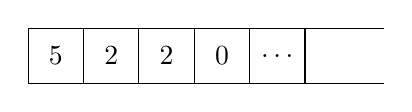
\begin{tikzpicture}[every node/.style={block},
        block/.style={minimum height=2em,minimum width=2em,outer sep=0pt,draw,rectangle,node distance=0pt}]
   \node (R1) {$5$};
   \node (R2) [right=of R1] {$2$};
   \node (R3) [right=of R2] {$2$};
   \node (R4) [right=of R3] {$0$};
   \node (R5) [right=of R4] {$\ldots$};
   \draw (R5.north east) -- ++(1cm,0) (R5.south east) -- ++ (1cm,0);
\end{tikzpicture}
\end{center}
\end{columns}
\end{frame}

\begin{frame}{Example}
\begin{columns}
\column{0.5\linewidth}
\begin{center}
\begin{algorithmic}[1]
\STATE {$J(2, 3, 69420)$}
\STATE {$S(1)$}
\STATE {$S(3)$}
\STATE {$J(1, 1, 1)$}
\end{algorithmic}
\end{center}
\column{0.5\linewidth}
\begin{center}
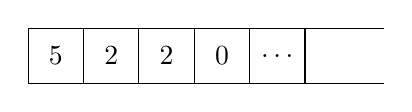
\begin{tikzpicture}[every node/.style={block},
        block/.style={minimum height=2em,minimum width=2em,outer sep=0pt,draw,rectangle,node distance=0pt}]
   \node (R1) {$5$};
   \node (R2) [right=of R1] {$2$};
   \node (R3) [right=of R2] {$2$};
   \node (R4) [right=of R3] {$0$};
   \node (R5) [right=of R4] {$\ldots$};
   \draw (R5.north east) -- ++(1cm,0) (R5.south east) -- ++ (1cm,0);
\end{tikzpicture}
\end{center}
4: $J(1, 1, 1)$

1: $J(2, 3, 69420)$

We now halt since the numbers in $R_2$ and $R_3$ are equal (both 2). We output 5, which is indeed $f(3, 2)$.
\end{columns}
\end{frame}

\begin{frame}{A useful tool}
\vspace{2mm}
Try it out yourself! \url{https://sites.oxy.edu/rnaimi/home/URMsim.htm}

\tiny

(Sorry Firefox users, it's time to whip out Microsoft Edge.)

Note: The website uses $T(m, n)$ instead of $C(m, n)$ to denote the copy instruction.

\begin{figure}
\includegraphics[scale=0.25]{img/ss1.png}
\end{figure}
\end{frame}

\begin{frame}{Now it's your turn!}
Let $f: \mathbb N \to \mathbb N$, $f(a) = 3a$. Build a URM to compute this function.

\vspace{6mm}

\small If you're done, try building a URM for this function:
$$f: \mathbb N \to \mathbb N, f(a) = \begin{cases}
0 & \text{$a$ even}\\
1 & \text{$a$ odd.}\\
\end{cases}$$
\end{frame}

\begin{frame}{Solution}
There are multiple different URMs that compute $f: \mathbb N \to \mathbb N$, $f(a) = 3a$. Example:
\begin{center}
\begin{algorithmic}[1]
\STATE {$S(5)$}
\STATE {$S(5)$}
\STATE {$C(1, 2)$}
\STATE {$J(2, 3, 8)$}
\STATE {$S(1)$}
\STATE {$S(3)$}
\STATE {$J(1, 1, 4)$}
\STATE {$Z(3)$}
\STATE {$S(4)$}
\STATE {$J(4, 5, 2020)$}
\STATE {$J(1, 1, 4)$}
\end{algorithmic}
\end{center}
\end{frame}

\begin{frame}{Turing machines!}
\sout{Now that you have the URM in the back of your mind, I can introduce Turing machines!}

actually nvm it would take way too much time. Here's the informal idea of a Turing machine (don't worry if you don't understand everything here):\footnote{There are many equivalent ways of defining the Turing machine. This may differ from what is defined in this class later.}

\vspace{2mm}

You have a tape, as before, but this tape extends infinitely in both directions.
You also have a \textit{read-write head}, pointing to a position on the tape.

\vspace{2mm}

Each position on the tape can store a symbol in a specified \textit{alphabet} (remember CSC236!). For example, our alphabet could be $\{0, 1\}$, or it could be the set of all ASCII characters. There is a specially designated \textit{empty symbol}, usually denoted by $0$, that the tape is filled with. 
\end{frame}

\begin{frame}{Turing machines!}
The Turing machine takes in a string input, say ``sushi''. The execution starts with ``sushi'' written on the tape (and $0$ everywhere else), and the read-write head pointing to the first letter of ``sushi''.

\begin{center}
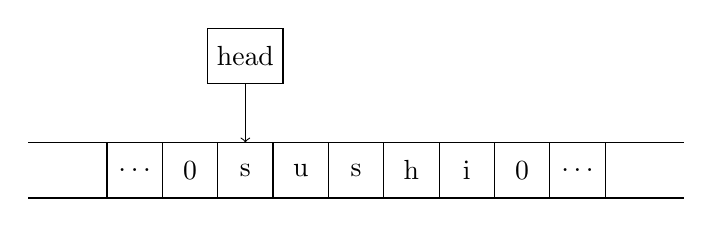
\begin{tikzpicture}[every node/.style={block},
        block/.style={minimum height=2em,minimum width=2em,outer sep=0pt,draw,rectangle,node distance=0pt}]
   \node (R1) {$\ldots$};
   \node (R2) [right=of R1] {$0$};
   \node (R3) [right=of R2] {s};
   \node (R4) [right=of R3] {u};
   \node (R5) [right=of R4] {s};
   \node (R6) [right=of R5] {h};
   \node (R7) [right=of R6] {i};
   \node (R8) [right=of R7] {$0$};
   \node (R9) [right=of R8] {$\ldots$};
   \node (HEAD) [above = 0.75cm of R3] {head};
   \draw[->] (HEAD) -- (R3);
   \draw (R1.north west) -- ++(-1cm,0) (R1.south west) -- ++ (-1cm,0);
   \draw (R9.north east) -- ++(1cm,0) (R9.south east) -- ++ (1cm,0);
\end{tikzpicture}
\end{center}
\end{frame}

\begin{frame}{Turing machines!}
The Turing machine also has a set of predetermined \textit{states}, which can be encoded in a DFA (from CSC236). Each state dictates the current behaviour of the Turing machine.

In each iteration of the Turing machine, we do the following:
\begin{enumerate}
\item Read the symbol, from the read-write head.
\item Inquire the current state: what should I do if I have read in this symbol? The current state will give us the following:
\begin{itemize}
\item A symbol to write back. (This symbol might be the same as the symbol we read in.)
\item A new state to transition to (which might be the same state).
\item A direction to move the read-write head in by one, either left or right (we \textbf{must} move the read-write head).
\end{itemize}
\end{enumerate}

In addition, the Turing machine specifies a starting state, and a list of halting states, just like in a DFA. After halting, the Turing machine outputs whatever is left on the tape.
\end{frame}

\begin{frame}{Turing machines!}
That was very informal. Here's the formal definition from Wikipedia:
\begin{figure}[h!]
\centering
\includegraphics[scale=0.15]{img/ss2.png}
\caption*{Greek letters scare people so that's why I didn't feel like giving a full overview of the Turing machine today, sowwy owo}
\end{figure}

The catchline is that although Turing machines are more complicated than URMs, whatever Turing machines can compute, URMs can also compute, and vice versa. So in some sense their ``computational power'' is equivalent! In fact, theoretically you could simulate a Turing machine inside a URM, and vice versa.

\end{frame}

\begin{frame}{Example of Turing machine!}
Let's make sushi! owo

\vspace{2mm}

Our alphabet will be $\left\lbrace 0, \emojifish, \emojirice, \emojisushi\right\rbrace$. The states in the DFA for the Turing machine will be 
$\left\lbrace \textit{empty}, \text{rice}, \text{fish}, \textbf{finish}, \textbf{fail}\right\rbrace$ with \textit{empty} being the starting state and bold states being halting states.

\vspace{2mm}

Remember, each state takes in a symbol from the alphabet and outputs three things: a symbol to write back, a new state to transition to, and a direction to move the read-write head.

\end{frame}

\begin{frame}{Example of Turing machine!}
Consider the following table:
\begin{table}
\begin{tabular}{c|c|c|c|c}
State & $0$ & \emojifish & \emojirice & \emojisushi\\
\hline
\textit{empty} & ($0$, \textbf{fail}, R) & (0, fish, R) & (0, \textbf{fail}, R) & - \\
\hline
fish & ($0$, \textbf{fail}, R) & ($0$, \textbf{fail}, R) & (\emojisushi, \textbf{finish}, R) & - \\
\hline
rice & ($0$, \textbf{fail}, R) & (\emojisushi, \textbf{finish}, R) & ($0$, \textbf{fail}, R) & - \\
\hline
\textbf{finish} & - & - & - & - \\
\hline
\textbf{fail} & - & - & - & - \\
\end{tabular}
\end{table}
where $-$ denotes that we will never encounter this symbol while in this state (if you wanna be formal, just put anything you want there)
\end{frame}

\begin{frame}{Example of Turing machine!}
Let's try executing our sushi machine on the string ``\emojifish\emojirice''!

\vspace{2mm}

Current State: \textit{empty}
\begin{center}
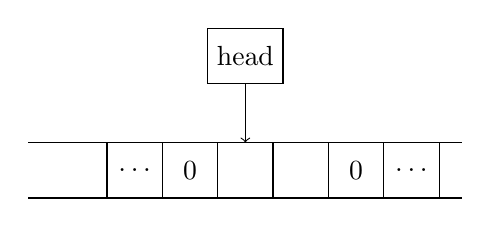
\begin{tikzpicture}[every node/.style={block},
        block/.style={minimum height=2em,minimum width=2em,outer sep=0pt,draw,rectangle,node distance=0pt}]
   \node (R1) {$\ldots$};
   \node (R2) [right=of R1] {$0$};
   \node (R3) [right=of R2] {\emojifish};
   \node (R4) [right=of R3] {\emojirice};
   \node (R5) [right=of R4] {$0$};
   \node (R6) [right=of R5] {$\ldots$};
   \node (HEAD) [above = 0.75cm of R3] {head};
   \draw[->] (HEAD) -- (R3);
   \draw (R1.north west) -- ++(-1cm,0) (R1.south west) -- ++ (-1cm,0);
   \draw (R5.north east) -- ++(1cm,0) (R5.south east) -- ++ (1cm,0);
\end{tikzpicture}
\end{center}
\end{frame}

\begin{frame}{Example of Turing machine!}
We read in \emojifish, and consult our current state \textit{empty}. 

\begin{table}
\begin{tabular}{c|c|c|c|c}
State & $0$ & \emojifish & \emojirice & \emojisushi\\
\hline
\textit{empty} & ($0$, \textbf{fail}, R) & (0, fish, R) & (0, \textbf{fail}, R) & - \\
\end{tabular}
\end{table}
Our current state returns ($0$, \text{fish}, R). So we write back $0$, go to the fish state, and move the head right.

\vspace{2mm}

Current State: fish
\begin{center}
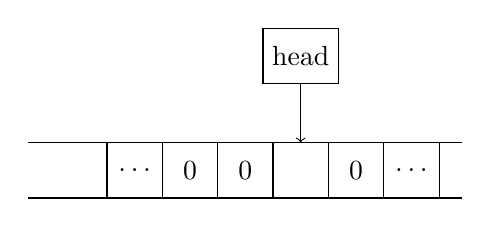
\begin{tikzpicture}[every node/.style={block},
        block/.style={minimum height=2em,minimum width=2em,outer sep=0pt,draw,rectangle,node distance=0pt}]
   \node (R1) {$\ldots$};
   \node (R2) [right=of R1] {$0$};
   \node (R3) [right=of R2] {$0$};
   \node (R4) [right=of R3] {\emojirice};
   \node (R5) [right=of R4] {$0$};
   \node (R6) [right=of R5] {$\ldots$};
   \node (HEAD) [above = 0.75cm of R4] {head};
   \draw[->] (HEAD) -- (R4);
   \draw (R1.north west) -- ++(-1cm,0) (R1.south west) -- ++ (-1cm,0);
   \draw (R5.north east) -- ++(1cm,0) (R5.south east) -- ++ (1cm,0);
\end{tikzpicture}
\end{center}
\end{frame}

\begin{frame}{Example of Turing machine!}
We read in \emojirice, and consult our current state fish. 

\begin{table}
\begin{tabular}{c|c|c|c|c}
State & $0$ & \emojifish & \emojirice & \emojisushi\\
\hline
fish & ($0$, \textbf{fail}, R) & ($0$, \textbf{fail}, R) & (\emojisushi, \textbf{finish}, R) & - \\
\end{tabular}
\end{table}
Our current state returns (\emojisushi, \textbf{finish}, R). So we write back \emojisushi, go to the \textbf{finish} state, and move the head right.

\vspace{2mm}

Current State: \textbf{finish}
\begin{center}
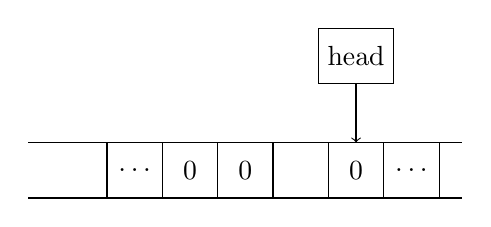
\begin{tikzpicture}[every node/.style={block},
        block/.style={minimum height=2em,minimum width=2em,outer sep=0pt,draw,rectangle,node distance=0pt}]
   \node (R1) {$\ldots$};
   \node (R2) [right=of R1] {$0$};
   \node (R3) [right=of R2] {$0$};
   \node (R4) [right=of R3] {\emojisushi};
   \node (R5) [right=of R4] {$0$};
   \node (R6) [right=of R5] {$\ldots$};
   \node (HEAD) [above = 0.75cm of R5] {head};
   \draw[->] (HEAD) -- (R5);
   \draw (R1.north west) -- ++(-1cm,0) (R1.south west) -- ++ (-1cm,0);
   \draw (R5.north east) -- ++(1cm,0) (R5.south east) -- ++ (1cm,0);
\end{tikzpicture}
\end{center}

Then we halt since \textbf{finish} is a halting state, and return \emojisushi! \emojisavouring
\end{frame}


\begin{frame}{bye!}
hope you learned something today!

i'll probably post the slides later, and set up a pateron to fund my sushi addiction.
\end{frame}


\begin{frame}{License}

  \begin{block}{Get the source of this theme and the demo presentation from}

  \begin{center}\url{http://github.com/famuvie/beamerthemesimple}\end{center}

  \end{block}
  
  The theme \emph{itself} is licensed under a
  \href{http://creativecommons.org/licenses/by-sa/4.0/}{Creative Commons
  Attribution-ShareAlike 4.0 International License}.

  \begin{center}\ccbysa\end{center}

\end{frame}

\end{document}